\documentclass[11pt,a4paper]{article}
\usepackage[margin=2.4cm]{geometry}
\usepackage[T1]{fontenc}
\usepackage[utf8]{inputenc}
\usepackage{lmodern}
\usepackage{amsmath,amssymb}
\usepackage{booktabs}
\usepackage{graphicx}
\usepackage{caption}
\usepackage{enumitem}
\usepackage{xcolor}
\usepackage{url}
\usepackage[hidelinks]{hyperref}
\usepackage{microtype}
\graphicspath{{figures/}}
\setlength{\parskip}{4pt}
\captionsetup{font=small,labelfont=bf}

\newcommand{\code}[1]{\texttt{#1}}
\newcommand{\HV}{\mathrm{HV}}
\newcommand{\IGD}{\mathrm{IGD}}

\title{\textbf{A Reproduction Study of LLM-NAS:\\ LLM-Driven Hardware-Aware Neural Architecture Search}\\[4pt]
\large Framework, data validation, and results on HW-NAS-Bench}
\author{Siyabonga Mjali\thanks{Implementation and experiments were carried out with AI-assisted tooling (Claude Code). All numbers are generated by the code in the accompanying repository and can be regenerated from the archived run logs.}}
\date{25 October 2026}

\begin{document}
\maketitle

\begin{abstract}
We report an independent reproduction of \emph{LLM-NAS: LLM-Driven Hardware-Aware Neural Architecture Search} (Zhu, Zhang \& Huang, 2025) on HW-NAS-Bench. No official code was available, so we implemented the method from the paper text, its Algorithm~1 and the prompts in its Appendix~E, inside a configuration-driven framework in which every LLM call is logged and replayable and every run is keyed by a hash of its configuration. Data-alignment checks show that our benchmark tables are the ones the paper used (11 of 12 reported Table-2 points are recovered exactly), and reveal one reported point that does not exist in the benchmark and a benchmark artefact (4{,}699 Edge-TPU latencies stored as $-1$) that corrupts hypervolume unless excluded. On the paper's headline setting (CIFAR-10, Edge GPU) the full method with GPT-4.1 reaches $\HV=0.964$ and $\IGD=0.063$ (one seed) against the paper's $0.997$ and $0.006$; with a local Qwen2.5-7B model it reaches $0.888$. Non-LLM controls run inside the paper's own niches reach $\HV=0.989\pm0.004$ (random evolution) and $0.991\pm0.001$ (random sampling) with no API calls. We therefore could \emph{not} reproduce an advantage of the LLM operator under our hypervolume convention; the paper does not state its normalisation or reference point, and we show that this unspecified convention is the dominant source of disagreement. We document every unspecified hyper-parameter and the choice made, list what was and was not reproduced, and propose the experiments that would resolve the remaining questions.
\end{abstract}

\tableofcontents
\newpage

%=====================================================================
\section{Introduction}
Hardware-aware neural architecture search (HW-NAS) seeks architectures that trade off task performance against on-device cost. Supernet-based methods are effective but cost GPU-days per dataset. LLM-NAS \cite{llmnas} replaces both the supernet and the evolutionary operator with a large language model that (a)~is confined to \emph{complexity niches} to counteract its tendency to repeat familiar designs (\emph{exploration bias}), (b)~co-evolves a textual \emph{knowledge base} of design rules alongside the architectures, and (c)~scores candidates with a training-free zero-cost (ZC) predictor. The paper reports near-perfect Pareto fronts (hypervolume $\approx0.99$) at a cost of 120 API calls per search.

This study has three goals:
\begin{enumerate}[nosep]
  \item Build an \emph{organised, re-runnable} reproduction: one command per paper table or figure, exact replay without API access, and an explicit record of every assumption.
  \item Validate that the benchmark data we use is the data the paper used.
  \item Run the method with the paper's LLM (GPT-4.1) and with an open 7B model (Qwen2.5-7B), and compare with the paper's reported numbers and with non-LLM controls.
\end{enumerate}
Section~\ref{sec:method} describes the method and framework, Section~\ref{sec:results} the results, Section~\ref{sec:discussion} what was discovered, and Section~\ref{sec:future} next steps. Appendix~\ref{sec:glossary} defines all technical terms and formulas.

%=====================================================================
\section{The method being reproduced}\label{sec:background}
The search space is the NAS-Bench-201 cell: six edges, each carrying one of five operators (\code{none}, \code{skip\_connect}, \code{nor\_conv\_1x1}, \code{nor\_conv\_3x3}, \code{avg\_pool\_3x3}), giving $5^6=15{,}625$ architectures. HW-NAS-Bench \cite{hwnasbench} supplies measured latency for every architecture on six devices (Edge GPU, Raspberry~Pi~4, Edge TPU, Pixel~3, Eyeriss, FPGA).

\paragraph{Complexity niches.} The space is partitioned into six disjoint niches by the number of $3{\times}3$ convolutions (Table~1 of the paper): S0 none and no $1{\times}1$; S1 none but at least one $1{\times}1$; S2, S3, S4 exactly one, two, three $3{\times}3$; S5 four or more. The niches contain 729, 3{,}367, 6{,}144, 3{,}840, 1{,}280 and 265 architectures respectively.

\paragraph{Search (Algorithm 1).} Each niche keeps its own Pareto archive over (predicted accuracy, latency). In each of 10 generations and for each niche the LLM is called twice: \emph{Stage~1} rewrites the knowledge base from the previous cycle's results; \emph{Stage~2} proposes children by crossover (two parents) or mutation (one parent) under the niche's constraint, with the knowledge base in the prompt. Children are evaluated, the niche archive is updated, and after the last generation the archives are merged and filtered by non-dominated sorting. This is $6\times10\times2=120$ calls.

\paragraph{Training-free evaluation.} Latency comes from the HW-NAS-Bench lookup table. Accuracy is predicted by an XGBoost regressor over the 13 zero-cost proxies of NAS-Bench-Suite-Zero \cite{nbsz}.

\paragraph{Metrics.} Hypervolume (HV) and inverted generational distance (IGD) of the discovered front against the true front (definitions in Appendix~\ref{sec:glossary}).

%=====================================================================
\section{Reproduction methodology}\label{sec:method}

\subsection{Framework}
The implementation is a Python package with the following properties, all motivated by the need to regenerate thesis numbers years later:
\begin{itemize}[nosep]
  \item \textbf{One configuration system.} \code{configs/base.yaml} holds every default, each tagged \code{[paper]} (stated in the paper) or \code{[assumed]} (our choice). Experiment files define a grid (datasets $\times$ devices $\times$ seeds) and named variants as overrides.
  \item \textbf{Content-addressed runs.} A run lives at \path{results/runs/<variant>-<hash8>/<dataset>/<device>/seed<k>/}, where the hash covers the effective configuration (excluding fields that cannot change results). A finished run is never recomputed, interrupted grids resume, and changing any setting creates a new directory rather than overwriting.
  \item \textbf{Replayable LLM calls.} Every prompt, response, token count and wall time is appended to \code{llm\_calls.jsonl}. Running with \code{llm.mode=replay} feeds the saved responses back and reproduces the run exactly (a mismatch counter must read zero); verified on the Qwen run, which replayed identically in 1.4\,s.
  \item \textbf{Provenance.} Each run records the git commit (with a dirty flag) that produced it.
  \item \textbf{Pluggable LLM backends.} Any OpenAI-compatible endpoint (GPT-4.1, OpenRouter, Ollama), Anthropic Claude, or an offline mock used only for tests.
  \item \textbf{Tests.} Unit and end-to-end tests run on synthetic data without the 2\,GB download, including searches with the mock backend and exact-replay checks.
\end{itemize}

\subsection{Data}
Three public sources were merged into one table per dataset (15{,}625 rows): HW-NAS-Bench v1.0 (latency); NAS-Bench-Suite-Zero \code{zc\_nasbench201.json} (13 ZC proxies and validation accuracy); and NATS-Bench \cite{nats} (200-epoch \emph{test} accuracy, which is what the paper's Table~2 reports, e.g.\ the 94.37\% CIFAR-10 optimum). NASLib encodes architectures with a different operator order and edge permutation from the NB201 string. The mapping (operators \code{[skip,none,conv3,conv1,pool]}, edge permutation $[0,1,3,2,4,5]$) was verified by matching validation accuracies on all 15{,}625 architectures.

\subsection{Predictor, metrics and variants}
\textbf{Predictor.} XGBoost (500 trees, depth 6, learning rate 0.05) on the 13 ZC proxies, trained on 1{,}000 random architectures labelled with NB201 \emph{validation} accuracy, predicts for the whole space once so that the search performs $O(1)$ lookups. The Synflow ablation (implemented, not run) maps the raw Synflow score to the accuracy scale by isotonic regression, leaving its ranking unchanged.

\textbf{Metrics.} Both objectives are minimised internally as (latency, $-$accuracy), normalised by the ideal and nadir points of the true front $P^\ast$, with reference point $r=(1.1,1.1)$. We report $\HV(S,r)/\HV(P^\ast,r)$ and $\IGD(S,P^\ast)$. The paper gives neither its normalisation nor its reference point; because it reports $\HV\le1$ and ``near-perfect'' values, a ratio is the most plausible reading.

\textbf{Variants.} Switches for each ablation: \code{partitioning} (six niches vs.\ the whole space), \code{operator} (\code{llm}; \code{random} = the paper's PEA ablation; \code{random\_sample} = uniform sampling within niches, our added floor), \code{knowledge\_base} on/off, and \code{predictor.kind}. Un-partitioned variants receive the same evaluation budget as partitioned ones. Prompts follow Appendix~E of the paper verbatim where text is given; the architecture legend and the parent tables fill the paper's placeholders.

\subsection{Unspecified details and the choices made}\label{sec:assumed}
\begin{table}[h]\centering\small
\caption{Choices not specified by the paper (all exposed in \code{configs/base.yaml}); these are the first things to vary in a sensitivity study.}\label{tab:assumed}
\begin{tabular}{p{4.6cm}p{4.0cm}p{6.2cm}}
\toprule
Item & Choice & Rationale \\
\midrule
Initial population per niche & 5 random architectures & Algorithm~1 samples but gives no size \\
Children per Stage-2 call & 4 & $6\times10\times4=240$ proposals over 120 calls \\
Parents shown per prompt & $\le6$ (half newest, rest random) & Fig.~4 shows both ``last cycle'' and ``random from archive'' \\
Crossover probability $p_c$ & each child slot assigned crossover w.p.\ 0.5 & reconciles Sec.~4.1 ($p_c{=}0.5$) with App.~E (LLM decides) \\
Knowledge-base scope & one per niche & Stage-1 prompt contains the niche definition \\
Invalid / duplicate / out-of-niche proposals & discarded, no retry, counted & keeps the 120-call budget fixed \\
\code{latency\_limit} in prompt & omitted & never given a value \\
Temperature & 0.7 & not stated \\
Predictor training set & 1{,}000 archs, validation labels & ``trained on a sample''; avoids test leakage \\
Accuracy for HV/IGD & NB201 200-epoch test accuracy & Table~2 reports the 94.37\% test optimum \\
Discovered set $S$ & final front of Algorithm~1 (chosen by predicted accuracy), re-scored with true accuracy & Algorithm~1 returns $P_{\text{final}}$ \\
HV/IGD normalisation & true-front min--max, $r=(1.1,1.1)$, HV as a ratio & paper reports $\HV\le1$ \\
Seeds & 3 for non-LLM runs; 1 for LLM runs & paper reports $\pm$ without a count \\
\bottomrule
\end{tabular}
\end{table}

%=====================================================================
\section{Results}\label{sec:results}

\subsection{Scope of what was run}
Table~\ref{tab:scope} states exactly which paper items were and were not reproduced. We report this explicitly because the LLM runs are expensive and were limited to one seed.
\begin{table}[h]\centering\small
\caption{Reproduction status by paper item.}\label{tab:scope}
\begin{tabular}{p{4.3cm}p{2.3cm}p{8.1cm}}
\toprule
Paper item & Status & What was done \\
\midrule
Table 1 (niches) & reproduced & niche sizes computed from the benchmark \\
Fig.~2 (encoding), Fig.~3 (parameter clusters) & reproduced & example rows matched to the benchmark; Fig.~3 regenerated \\
Table 2 (selected architectures) & checked & 11/12 LLM-NAS points located in the benchmark (Sec.~\ref{sec:align}) \\
Table 3 (HV/IGD, 3 datasets $\times$ 6 devices) & \emph{one slice} & CIFAR-10/Edge GPU only, GPT-4.1 and Qwen, 1 seed each \\
Table 4 (search cost) & measured & tokens, calls and time recorded for the runs above \\
Table 5, Figs.~6--8 (ablations) & \emph{partial} & non-LLM variants (PEA, random sampling) on CIFAR-100, 6 devices, 3 seeds; the full-model and Synflow rows were not run \\
Figs.~1, 9 (exploration bias) & implemented, not run & \code{fig1\_bias} experiment exists \\
Sec.~4.4, Table 6, Fig.~5 (ViT) & not reproduced & needs an AutoFormer supernet and A6000 timing \\
Baselines (FairNAS, PRP-NAS, LLMatic, DARTS) & quoted & GPU-days of training each \\
\bottomrule
\end{tabular}
\end{table}

\subsection{Data-alignment checks}\label{sec:align}
\begin{itemize}[nosep]
  \item Best test accuracies match NB201 exactly: 94.37 / 73.51 / 47.31 (CIFAR-10 / CIFAR-100 / ImageNet16-120).
  \item \textbf{11 of the 12} LLM-NAS points in the paper's Table~2 exist in the benchmark with matching accuracy \emph{and} latency. The exception is Edge GPU ``94.37\% @ 4.35\,ms'': the 94.37\% architecture \code{(3,3,3,1,3,2)} runs at 6.81\,ms on Edge GPU, and no architecture has that pair. The identical row is printed for PRP-NAS-BA, suggesting a transcription error.
  \item All five example rows in the paper's Figure~2 match CIFAR-100/Edge GPU to within rounding, confirming the paper's 6-tuple encoding.
  \item \textbf{Benchmark artefact.} HW-NAS-Bench stores $-1$ as the Edge TPU latency of 4{,}699 architectures (30\%); the other five devices are complete. Treated as real values, these create fake zero-cost points on the ``true'' front and collapse Edge TPU hypervolume to $\approx0.2$ for every method; treated as unmeasured (our choice), Edge TPU behaves like the other devices ($\HV\approx0.92$). The paper does not say how it handled this.
  \item The ZC-ensemble predictor reaches Spearman $0.960\pm0.001$, $0.964\pm0.001$ and $0.957\pm0.002$ against test accuracy on the three datasets, above the paper's $\approx0.90$; Synflow alone reaches 0.75--0.78.
\end{itemize}

\subsection{Main comparison: CIFAR-10, Edge GPU}
Table~\ref{tab:cnn} and Figure~\ref{fig:cnnfronts} compare the full method under two LLMs with the non-LLM controls on the paper's headline setting. GPT-4.1 was run once (120 calls, 8.6\,min, 160{,}319 input and 66{,}747 output tokens, $\approx\$0.85$ at list price). Qwen2.5-7B (4-bit, Ollama, 8K context) was run once on an RTX~3050~Ti laptop GPU (153\,min, 129{,}207 input and 56{,}447 output tokens). The controls were run with three seeds.

\begin{table}[h]\centering\footnotesize
\caption{CIFAR-10, Edge GPU. HV$\uparrow$ as a fraction of the true front's HV; IGD$\downarrow$ in normalised units. ``Usable'' = proposals that were valid, inside their niche and not duplicates; ``Eval.'' = distinct architectures evaluated (both are means over seeds for the controls). Paper values from its Table~3, which also reports FairNAS 0.892\,/\,0.073, PRP-NAS 0.843\,/\,0.116 and LLMatic 0.191\,/\,0.542 (HV\,/\,IGD).}\label{tab:cnn}
\begin{tabular}{llccccc}
\toprule
Method & LLM & Seeds & HV & IGD & Usable & Eval. \\
\midrule
LLM-NAS (paper) & GPT-4.1 & ? & 0.997 & 0.006 & -- & -- \\
LLM-NAS (ours) & GPT-4.1 & 1 & 0.964 & 0.063 & 99/240 (41\%) & 129 \\
LLM-NAS (ours) & Qwen2.5-7B & 1 & 0.888 & 0.088 & 95/240 (40\%) & 125 \\
PEA: niches, random operators & -- & 3 & $0.989\pm0.004$ & $0.038\pm0.008$ & 155/240 (65\%) & 185 \\
Random sampling in niches & -- & 3 & $0.991\pm0.001$ & $0.052\pm0.012$ & 239/240 (100\%) & 269 \\
\bottomrule
\end{tabular}
\end{table}

\begin{figure}[h]\centering
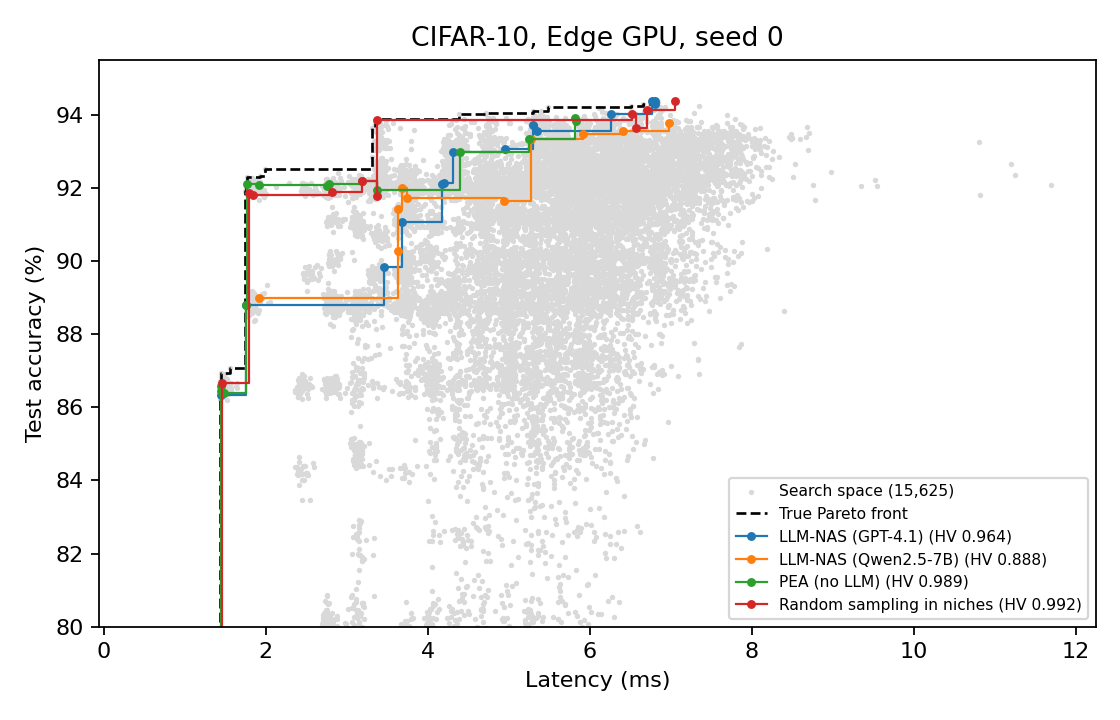
\includegraphics[width=0.8\textwidth]{cnn_fronts_edgegpu.png}
\caption{Final fronts on CIFAR-10 / Edge GPU (seed 0) against the true Pareto front. Both LLM variants miss the fastest region of the front; GPT-4.1 does recover the 94.37\% optimum.}\label{fig:cnnfronts}
\end{figure}

Three observations follow. First, GPT-4.1 improves on Qwen (0.964 vs.\ 0.888), and its knowledge base contains sensible rules (e.g.\ for niche S3: ``maintain exactly two \code{nor\_conv\_3x3} \ldots assign them to later or output-related edges''), but it still discards 59\% of its own proposals, 107 of them as duplicates of architectures it had already been shown. Second, both LLM variants are dominated by random proposals \emph{inside the same niches}, which reach $\HV\approx0.99$ with no API calls. Third, the HV trajectories (seed 0: GPT-4.1 $0.883\!\to\!0.964$ in a single jump at generation~7; random sampling $0.883\!\to\!0.990$ by generation~5) show that the initial 30 random samples already reach $\HV=0.883$ under this normalisation, leaving only $\approx0.11$ of head-room for any search procedure.

\subsection{Cost}
The paper reports 3 minutes and 120 API calls per search. Our GPT-4.1 run made 120 calls and took 8.6 minutes (about 4\,s per call, API latency included). At the measured token counts one search costs about \$0.85, so the paper's full Table-3 grid (18 settings, 3 seeds) would cost roughly \$46 with GPT-4.1. Qwen2.5-7B on a 4\,GB laptop GPU is free but slow: about 70--90\,s per call, i.e.\ 2.5\,h per search.

\subsection{Ablation on CIFAR-100 (paper's Table 5)}
The paper reports that removing the LLM operator (PEA) lowers average HV on CIFAR-100 from 0.978 to $0.843\pm0.075$. We could only run the non-LLM variants. With our normalisation, PEA achieves $0.946\pm0.031$ averaged over the six devices (three seeds each), and uniform random sampling within niches $0.931\pm0.047$ (Table~\ref{tab:abl}, Figure~\ref{fig:abl}). Our PEA is $\approx0.10$ above the paper's PEA, a gap as large as the one the paper attributes to the LLM. The HV convention, not the operator, is therefore the dominant unknown. We also noticed that the paper's Table-5 average HV for the full model (0.978) is not the mean of its six Table-3 CIFAR-100 values (0.982), although the IGD average does match.

\begin{table}[h]\centering\small
\caption{CIFAR-100, non-LLM variants, mean over 3 seeds. Edge TPU is scored after excluding unmeasured latencies.}\label{tab:abl}
\begin{tabular}{lcccccccc}
\toprule
 & \multicolumn{6}{c}{HV$\uparrow$ per device} & \multicolumn{2}{c}{Average} \\
\cmidrule(lr){2-7}\cmidrule(lr){8-9}
Variant & EGPU & Pi4 & ETPU & Pix3 & Eyer. & FPGA & HV & IGD \\
\midrule
PEA (random operators) & 0.979 & 0.974 & 0.916 & 0.976 & 0.926 & 0.904 & 0.946 & 0.062 \\
Random sampling in niches & 0.976 & 0.978 & 0.903 & 0.977 & 0.875 & 0.878 & 0.931 & 0.061 \\
Paper: PEA (Table 5) & \multicolumn{6}{c}{--} & 0.843 & 0.165 \\
\bottomrule
\end{tabular}
\end{table}

\begin{figure}[h]\centering
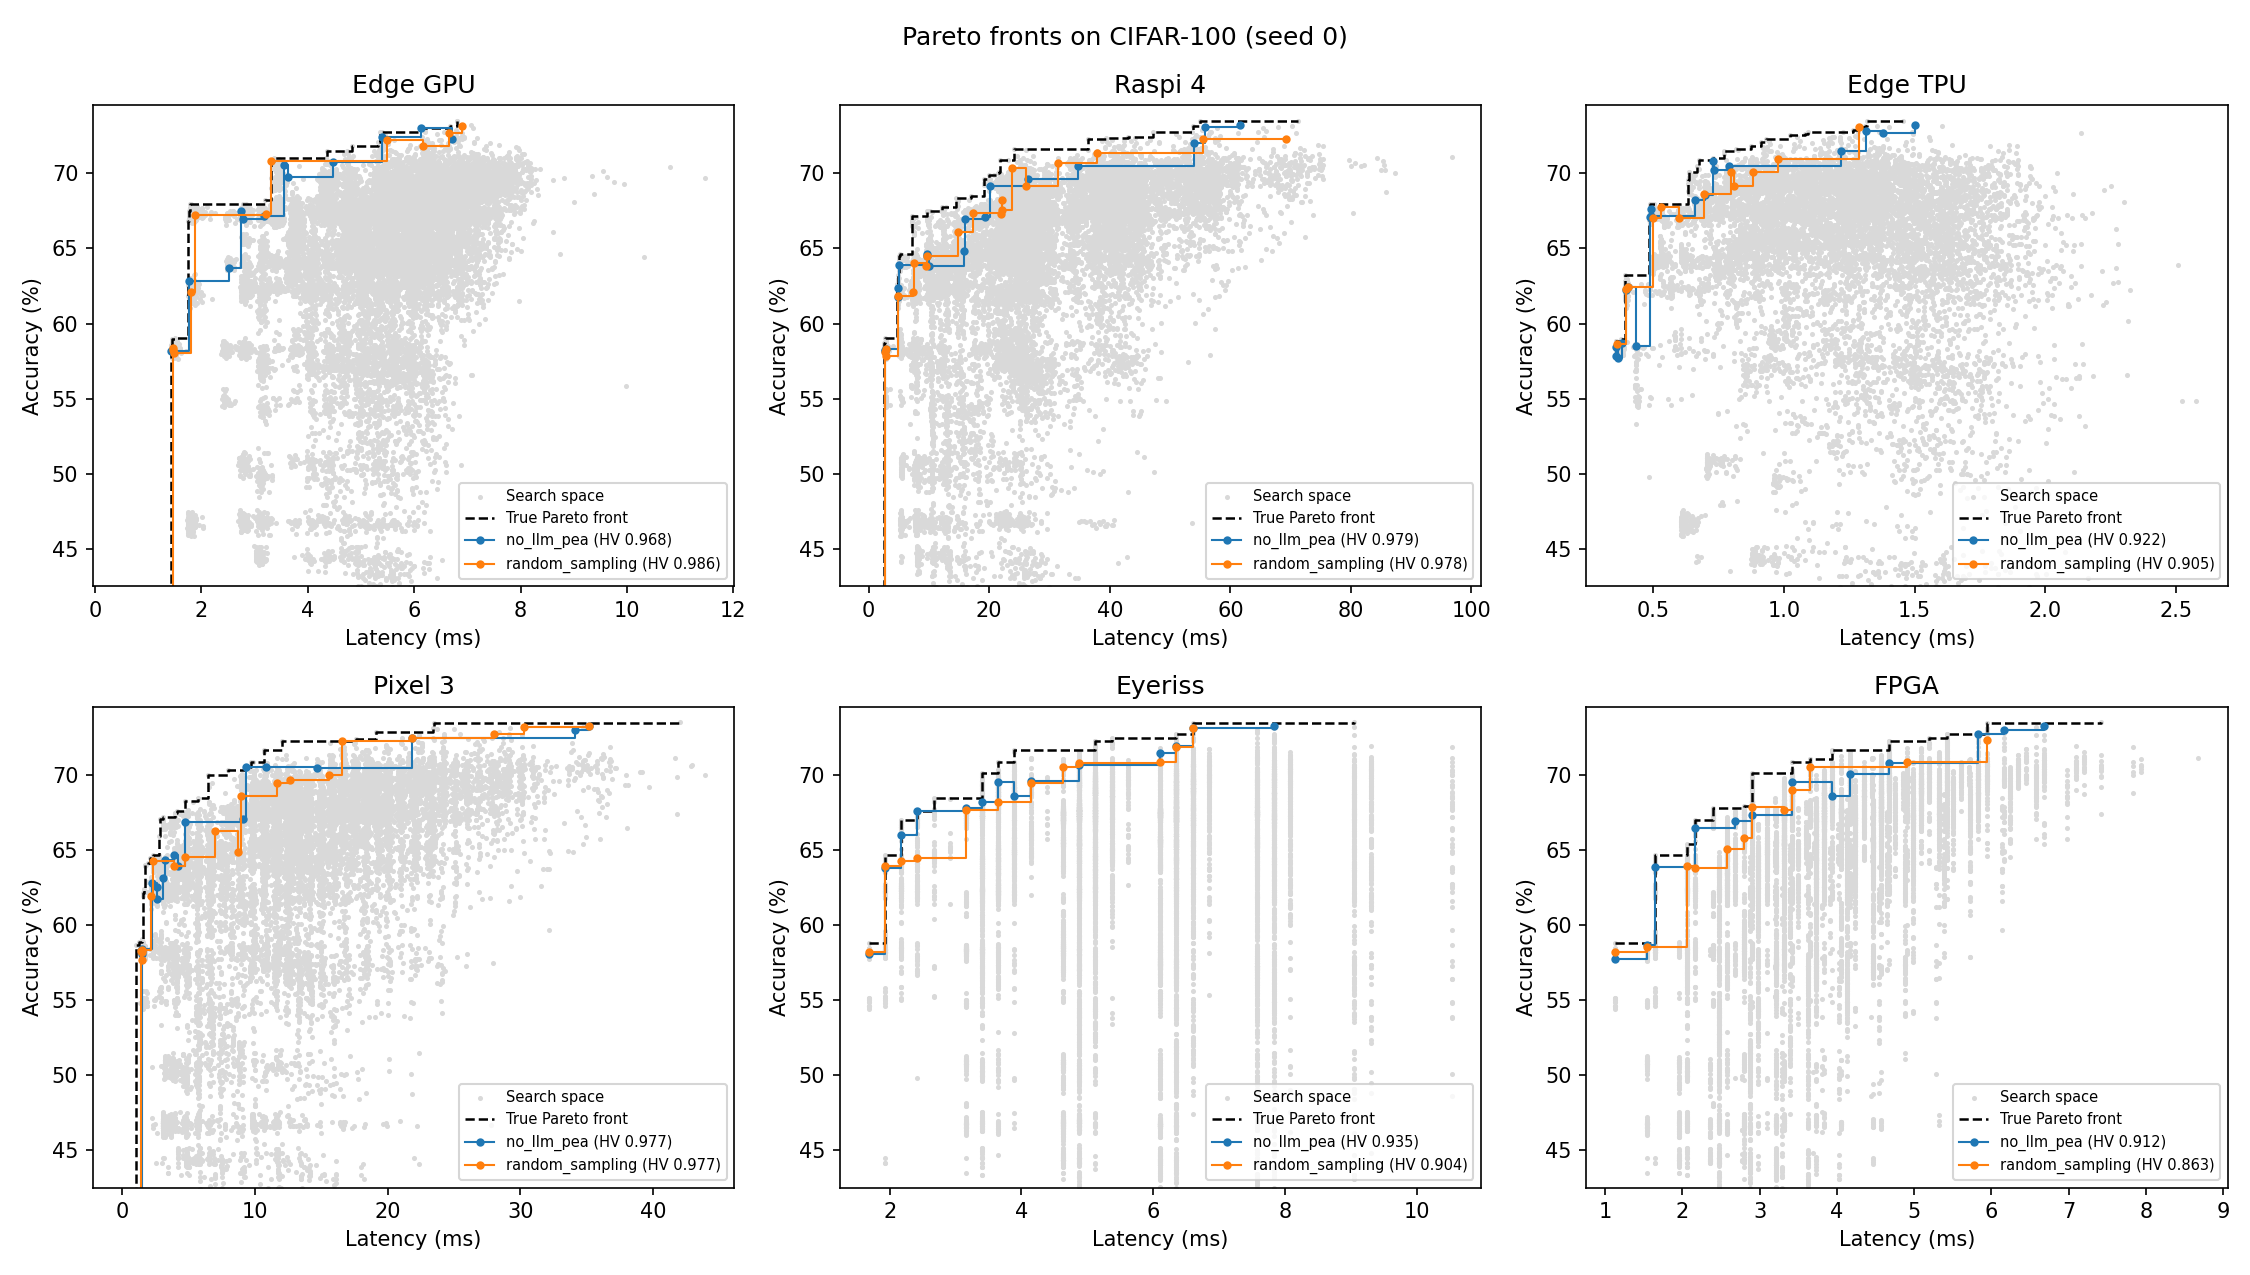
\includegraphics[width=\textwidth]{fronts_cifar100.png}
\caption{Non-LLM fronts on CIFAR-100 for all six devices (seed 0).}\label{fig:abl}
\end{figure}

%=====================================================================
\section{Discussion: what was discovered}\label{sec:discussion}
\begin{enumerate}
  \item \textbf{The paper's data and encoding are recoverable, with two caveats.} Eleven of twelve Table-2 points are reproduced exactly; one (Edge GPU 94.37\% @ 4.35\,ms) does not exist in HW-NAS-Bench. The Edge TPU column contains 4{,}699 placeholder values that must be excluded; this is not mentioned in the paper and materially changes Edge TPU numbers.
  \item \textbf{The HV convention is the dominant unknown.} Under the natural normalisation, 30 random samples already reach $\HV=0.88$ and random sampling within niches reaches $0.99$. The paper's reported gaps (full model 0.978 vs.\ PEA 0.843 on CIFAR-100) cannot be reproduced without a convention that penalises coverage gaps more heavily than ours. Until the authors specify their reference point and normalisation, HV comparisons across papers in this space are not meaningful.
  \item \textbf{We did not reproduce an advantage of the LLM operator.} With GPT-4.1 (one seed) HV is 0.964 against 0.989--0.991 for non-LLM controls inside the same niches; with Qwen2.5-7B it is 0.888. The mechanism is visible in the proposal statistics: 59--60\% of LLM proposals are discarded as out-of-niche or duplicate, so the LLM evaluates roughly half as many new architectures as the controls for the same budget. This is a statement about our conventions and budget, not a refutation of the paper (see Section~\ref{sec:threats}).
  \item \textbf{The LLM's knowledge base is meaningful but not self-correcting.} GPT-4.1 produced interpretable, mostly sensible rules about operator placement and latency; the weaker model produced rules that the data contradicted, and the co-evolution loop did not reliably remove them.
  \item \textbf{Capability matters.} GPT-4.1 outperforms Qwen2.5-7B (0.964 vs.\ 0.888) with a lower rate of out-of-niche proposals (14\% vs.\ 30\%), consistent with the idea that the method's benefit depends on the model, but one seed each cannot establish it.
\end{enumerate}

\section{Threats to validity}\label{sec:threats}
\begin{itemize}[nosep]
  \item \textbf{One seed for each LLM run, one dataset/device.} The paper's own LLM was run once on one setting because of budget; the seed-to-seed spread of LLM runs is unknown and could be several hundredths of HV.
  \item \textbf{A local 7B model is not the paper's setting.} Qwen results are a reproduction with a substituted LLM and are reported as such.
  \item \textbf{Assumed hyper-parameters} (Table~\ref{tab:assumed}). The number of children per call, the predictor training size and the parent-selection rule are plausible drivers of the remaining gap.
  \item \textbf{Stronger predictor than the paper's} (Spearman 0.96 vs.\ 0.90): it should help all methods equally but is a difference.
  \item \textbf{Unspecified HV/IGD convention} (Section~\ref{sec:method}); every HV and IGD comparison with the paper's numbers inherits this uncertainty.
  \item \textbf{Partial ablation.} The CIFAR-100 ablation lacks the full-model and Synflow rows, so the paper's Table~5 gaps cannot be checked directly.
\end{itemize}

%=====================================================================
\section{Future work}\label{sec:future}
Ordered by cost and by how much each would change the conclusions:
\begin{enumerate}
  \item \textbf{Obtain the paper's HV/IGD convention from the authors} (reference point, normalisation, whether $S$ is the archive or all evaluated architectures) and re-score the archived runs. Zero cost; the replay logs make this a one-line change.
  \item \textbf{GPT-4.1, three seeds, CIFAR-10 on all six devices} (6 devices $\times$ 3 seeds $\times$ 120 calls $\approx$ 2{,}160 calls, $\approx\$15$), then the CIFAR-100 and ImageNet16-120 slices to complete Table~3 (full grid $\approx\$46$). This decides whether finding~3 is a model-capability effect or a property of the method, and gives the seed-to-seed spread.
  \item \textbf{Complete the CIFAR-100 ablation} with the full-model and Synflow variants, so that Table~5 can be compared row by row.
  \item \textbf{Reduce proposal waste and re-test.} Three cheap interventions, each one configuration flag: (a)~reject-and-retry out-of-niche proposals within the same call; (b)~show the LLM the full evaluated set, not only the parents, to reduce duplicates; (c)~schema-constrained decoding with the niche's operator counts enforced. If the LLM operator still trails random sampling once its usable rate matches the controls', the negative result is robust.
  \item \textbf{Sensitivity study on the assumed hyper-parameters} (children per call $\in\{2,4,8\}$, predictor $n_{\text{train}}\in\{200,1000,5000\}$, parents shown), reported with the alternative HV conventions.
  \item \textbf{Run the exploration-bias experiment} (the paper's Figures~1 and 9; implemented, 10--20 calls per device) to test the paper's motivating claim directly.
  \item \textbf{More LLMs at a fixed budget} (GPT-4.1-mini, Claude Sonnet~5.5, a 14B local model) to map the capability-versus-benefit curve suggested by the GPT-4.1/Qwen gap.
  \item \textbf{Re-run a baseline} (e.g.\ a NAS-Bench-201 supernet or PRP-NAS if code is available) so that the quoted baseline numbers are on the same footing as ours.
  \item \textbf{Vision-Transformer experiment} (Section~4.4 of the paper), which needs an AutoFormer supernet, the ViT-Bench-101 predictor and latency profiling on a GPU.
\end{enumerate}

\section{Reproducibility and artefacts}
All code, configurations and reports are in the \code{llm-nas-repro} repository. Benchmark data (2\,GB) is re-created by \code{python -m llmnas prepare-data}. The archived \path{results/runs/} directory (per run: \code{config.yaml}, \code{run.json}, \code{llm\_calls.jsonl}) is the evidence behind every number in this report; \code{python -m llmnas report <experiment>} regenerates the tables and figures, and \code{--set llm.mode=replay} re-executes any LLM search without API access. A Colab notebook performs the same steps with data and results on Google Drive. Each run records the commit that produced it: the GPT-4.1 run used commit \code{1b5cf55}, the Qwen run and the non-LLM controls \code{bd5df23} (both 2 October 2026); neither commit changes the search or metric code relative to the other.

%=====================================================================
\appendix
\section{Glossary of terms and formulas}\label{sec:glossary}
\begin{description}[style=nextline,leftmargin=0pt,itemsep=3pt]

\item[Architecture code (NB201).] A 6-tuple $(a,b,c,d,e,f)\in\{0,\dots,4\}^6$ giving the operator on each edge of the 4-node cell in the order $n_1{\leftarrow}n_0,\ n_2{\leftarrow}n_0,\ n_2{\leftarrow}n_1,\ n_3{\leftarrow}n_0,\ n_3{\leftarrow}n_1,\ n_3{\leftarrow}n_2$, with $0$=\code{none}, $1$=\code{skip\_connect}, $2$=\code{nor\_conv\_1x1}, $3$=\code{nor\_conv\_3x3}, $4$=\code{avg\_pool\_3x3}.

\item[Configuration hash.] SHA-1 (first 8 hex digits) of the canonical JSON of a run's effective configuration, excluding fields that cannot affect results. Identical settings map to the same run directory.

\item[Crossover / mutation.] Evolutionary operators. Uniform crossover copies each gene from parent $A$ or $B$ with probability $\tfrac12$; mutation changes the operator on one edge.

\item[Exploration bias / mode collapse.] The tendency of a generative model to repeatedly propose a narrow family of outputs; LLM-NAS's motivation for niching.

\item[Hypervolume (HV).] For a set $S$ of points in $m$-objective space (minimisation) and a reference point $r$ dominated by all of $S$,
\[
\HV(S,r)=\lambda\Big(\bigcup_{s\in S}[s_1,r_1]\times\cdots\times[s_m,r_m]\Big),
\]
the Lebesgue measure of the dominated region. We report the ratio $\HV(S,r)/\HV(P^\ast,r)$ after min--max normalising each objective by the ideal and nadir points of the true front $P^\ast$, with $r=(1.1,1.1)$. In two dimensions it is computed by sorting the front by latency and summing rectangles.

\item[Inverted generational distance (IGD).]
\[
\IGD(S,P^\ast)=\frac{1}{|P^\ast|}\sum_{p\in P^\ast}\min_{s\in S}\lVert p-s\rVert_2,
\]
the mean distance from each true-front point to its nearest discovered point (normalised objectives). Lower is better; zero iff $S\supseteq P^\ast$.

\item[Isotonic regression.] Monotone non-decreasing least-squares fit; used to map Synflow scores to the accuracy scale without changing their ranking.

\item[Knowledge base (co-evolve).] A list of natural-language rules of the form ``use/avoid \ldots because \ldots'' that the LLM rewrites after each generation from the previous cycle's results and that is injected into the next generation prompt.

\item[Min--max normalisation.] $\tilde{x}_j=(x_j-\min_j)/(\max_j-\min_j)$ per objective $j$, with the extremes taken over the true front, so that normalised objectives lie in $[0,1]$ on the front.

\item[NAS-Bench-201 / NATS-Bench / HW-NAS-Bench / NAS-Bench-Suite-Zero.] Tabular benchmarks. NB201 (= NATS-Bench topology space) gives trained accuracy for all 15{,}625 cells on CIFAR-10/100 and ImageNet16-120; HW-NAS-Bench adds measured latency and energy on six devices; NAS-Bench-Suite-Zero adds 13 zero-cost proxy scores per architecture.

\item[Niche (partitioning).] A disjoint subset of the search space defined by the number of $3{\times}3$ convolutions (Table~1 of the paper). Each niche keeps its own Pareto archive; archives are merged by non-dominated sorting at the end.

\item[Pareto dominance / front.] For minimisation, $a\preceq b$ iff $a_j\le b_j\ \forall j$ and $a_j<b_j$ for some $j$. The Pareto front is the set of non-dominated points; the \emph{true front} $P^\ast$ is the front of all 15{,}625 architectures (excluding unmeasured latencies).

\item[PEA (partitioned evolutionary algorithm).] The paper's ``without LLM operator'' ablation: the same niches, archives and budget, with random mutation and crossover in place of the LLM.

\item[Replay.] Re-execution of a search with LLM responses taken from the saved call log instead of the API; must reproduce the original run exactly (mismatch counter 0).

\item[Seed.] Integer fixing a run's pseudo-random choices (initial population, predictor training sample, parent selection, crossover/mutation assignment, and the LLM sampling hint). Different seeds give independent repeats; results are reported as mean $\pm$ standard deviation over seeds.

\item[Spearman / Kendall rank correlation.] $\rho=1-\frac{6\sum d_i^2}{n(n^2-1)}$ over rank differences $d_i$ (Spearman); $\tau=\frac{C-D}{\binom{n}{2}}$ over concordant and discordant pairs (Kendall). Used to validate the predictor against ground truth.

\item[Usable proposal rate.] Fraction of LLM (or operator) proposals that parse, satisfy the niche constraint and are not duplicates of already-evaluated architectures; the remainder consume budget without producing an evaluation.

\item[XGBoost.] Gradient-boosted decision-tree regressor; here 500 trees of depth 6, learning rate 0.05, trained on the 13 ZC proxies.

\item[Zero-cost (ZC) proxy.] A score computed from an untrained network (one forward/backward pass or less) that correlates with trained accuracy, e.g.\ \code{synflow}, \code{snip}, \code{grasp}, \code{fisher}, \code{jacov}, \code{nwot}, \code{zen}, \code{epe\_nas}, \code{grad\_norm}, \code{l2\_norm}, \code{plain}, \code{params}, \code{flops}.
\end{description}

\begin{thebibliography}{9}
\bibitem{llmnas} H.~Zhu, G.~L.~Zhang, S.~Huang. LLM-NAS: LLM-Driven Hardware-Aware Neural Architecture Search. \emph{arXiv:2510.01472v4}, 2025.
\bibitem{hwnasbench} C.~Li et al. HW-NAS-Bench: Hardware-Aware Neural Architecture Search Benchmark. \emph{ICLR}, 2021.
\bibitem{nbsz} A.~Krishnakumar, C.~White, A.~Zela, R.~Tu, M.~Safari, F.~Hutter. NAS-Bench-Suite-Zero: Accelerating Research on Zero Cost Proxies. \emph{NeurIPS Datasets and Benchmarks}, 2022.
\bibitem{nats} X.~Dong, L.~Liu, K.~Musial, B.~Gabrys. NATS-Bench: Benchmarking NAS Algorithms for Architecture Topology and Size. \emph{IEEE TPAMI}, 2021.
\end{thebibliography}

\end{document}
